\section{Life cycle and roles}
In this section we go through the life cycle of a game, from idea through creation to a playable augmented board game. We focus on the roles and their contributions and actions in creating and using the game, as was the case with the previous augmented board game created at NTNU, Don't Panic . In the next section we will look at the challenges linked with these activities. 

We have identified three roles: a \textbf{Game Designer}, who formalizes and defines the game. The end result from a game designers production is a playable paper prototype. A \textbf{Developer} takes this prototype and identifies and acquires suitable hardware pieces, designs the user interface to be used in the game controller and implements the game through the controller and the hardware tokens. A \textbf{Player} should then able to acquire, set up and play the game. These roles and their typical activities are illustrated in figure \ref{fig:LifeCycleGameDesigner}, \ref{fig:LifeCycleDeveloper} and \ref{fig:LifeCyclePlayer}. The activites that we will focus on in this thesis is marked in green.



\begin{figure}[ht]
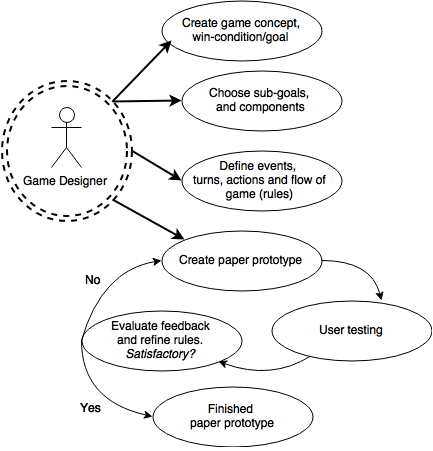
\includegraphics[width=8cm]{img/LifeCycleGameDesigner}
\centering
\caption{An overview over the responsibilities of the Game Designer in implementing hybrid board games. }
\label{fig:LifeCycleGameDesigner}
\end{figure}

\begin{figure}[ht]
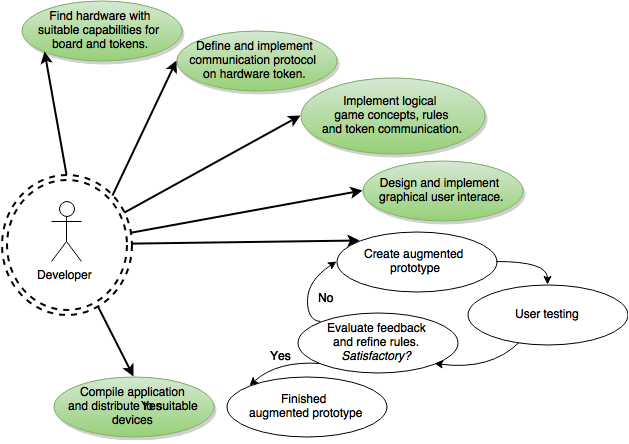
\includegraphics[width=12cm]{img/LifeCycleDeveloper}
\centering
\caption{An overview over the responsibilities of the Developer in implementing hybrid board games, after a finished paper prototype is provided by the game designer. The responsibilites marked with green are areas where we think AnyBoard can assist.}
\label{fig:LifeCycleDeveloper}
\end{figure}

\begin{figure}[ht]
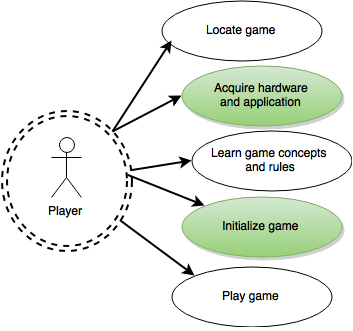
\includegraphics[width=7cm]{img/LifeCyclePlayer}
\centering
\caption{Main interactions from the view of a player in using hybrid board games. From previous experience in the testing of Don't Panic, replacing hardware tokens and game initialization (marked green) was too hard for non-technical players to receive a copy of the game.}
\label{fig:LifeCyclePlayer}
\end{figure}

\subsection{Designing}
The Game Designer starts with an idea, and details it through defining concepts, providing a motivation/goal, and giving the game clear rules and boundaries. The end result from the game designer should be a playable paper prototype of the board game. The following questions are the main questions that a game designer should be able to provide answers for (short Monopoly example answer in emphazised text):
\begin{enumerate} \label{design_cycle}
\item How are the teams - who is playing against who? \emph{Every player for themselves}
\item What is the game concept? Why are the players playing for/the goal? \emph{Achieving monopoly by making your opponents bankrupt}
\item What resources and game objects does the game consist of? Which is manifested in physical tokens? \emph{Stock, Money, Pawns, Houses, Hotel, Board, Question Cards}
\item What are the definite win- and lose conditions? \emph{You lose when you have no valuables left. Winner is the last player standing}
\item Through which actions does the game progress? \emph{Roll dice to change tiles. Tiles can be bought, traded, trigger event, paid rent for staying at. Each player takes it turn to complete a set of actions}
\item What are the initial set-up conditions of the game? \emph{Every player start at go tile with the same initial amount of resources.}
\end{enumerate}
These answers is described in detail and usually goes through several iterations (often with user feedback), before he or she comes to a final version that should be able to be played on a paper prototype. This iteration and refinement process could also be skipped, and rather done in the next phase, after implementating the game as an augmented board game.

\subsection{Implementing}
The Developer should have a clear description of the board game from the Game Designer. He will convert the game into an augmented version, by indentifying suitable digital tokens and interfaces, and implement the game logic into the necessary tokens and devices. A user friendly interface is necessary to allow players to initiate and play the game, and the applications should be distributed in a way that makes it easy to acquire. In short, the Developer takes the game from a finished concept to a finished product. This is shown in figure  \ref{fig:LifeCycleDeveloper}.

We have here assumed a case where a game controller (Phone, Tablet, Computer) and a set of tangible, digital hardware tokens has been used to create an augmented version of the board game. The Developers main responsibilites, are (examples are shown in emphasized text):
\begin{enumerate} \label{develop_cycle}
\item Translate the required token expressions and interactions into a clear grammar. \emph{Pawn can be placed on board and should notify of location. Pawn can show color and vibrate.}
\item Find or make digital hardware tokens that are capable of necessary token expressions. \emph{"rfduino" device should be capable of our requirements.}
\item Define and implement a communication protocol between tokens. \emph{Make "rfduino" accept "SET COLOR RED" over serial bluetooth and execute the corresponding expression.}
\item Implement game concepts, rules and token communication. \emph{Creating the logical representations of "Stock", "Money", "Board" etc, a token communicator object, and procedures to initiate the game and handle "paying rent".}
\item Designing and implementing the GUI. \emph{Creating a menu with buttons to run initiate procedure, read rules, and exit game. Designing an choice screen to handle trades between players}
\item Compile the game so it is distributable. \emph{Compile to iOS and Android files and distribute on App Store and Google Play}
\end{enumerate}
Prior to the compiling and distribution the game, the Developer should go through an iteration and refinement process to ensure the quality of the game. The game should now be ready for players to acquire and play the game.

\subsection{Playing}
A Player of the game is not involved in the creation of the game, but is a consumer of the finished product, a player of the augmented boardgame. In acquiring and playing the game, he or she will typically go through the following steps (examples in emphazised text, illustrated in figure \ref{fig:LifeCyclePlayer}):
\begin{enumerate} \label{play_cycle}
\item Locate the game. \emph{Hear of game from a friend, and go to its website.}
\item Acquire hardware and application. \emph{Order the necessary tokens online, and download a corresponding application from App Store}
\item Learn game rules. \emph{Read the game manual, and a FAQ on the applications website}
\item Initiate Game. \emph{Turn on tokens, open phone application, establish communication between tokens, and set up initial game conditions}
\item Play game. \emph{Interact with tokens (and phone application) according to the game rules}
\end{enumerate}



